\chapter{Reconhecimento de Expressões Faciais}

\section{Introdução}
Segundo \citeonline{FernandoGil} a expressão facial é uma forma de comunicação não-verbal que permite a partilha de
sentimentos e emoções, numa linguagem subentendida entre seres humanos. Desde o início das pesquisas na computação busca-se cada vez mais dotar o computador de um comprtamento inteligente. Sequindo esse caminho, o reconhecimento facial surgiu,  para trazer soluções no campo da Interface Homem- Computador, como um desafio esperado, porém desafiador. Principalmente no reconheciemnto de expressões faciais, já que se trata de um julgamento ambíguo até mesmo para os seres humanos, pois a mesma expressão pode variar de indivíduo para indivíduo \cite{FernandoGil} \cite{Elizabeth}.

\section{Fases do Reconhecimento}
O reconhecimento facial se divide em três etapas básicas \cite{Elizabeth}:
\begin{itemize}
\item Detectar a face na cena: Inicialmente é apresentada uma imagem contendo a face que deve ser rceonhecida. Nesta primeira etapa, deve ser realizada a detecção da zona da face, e devem ser extraídos os outros artefatos que não compõem o rosto \cite{FernandoGil}.
Na figura \ref{img:rosto} é ilustrado o resultado final desta primeira etapa.
\begin{center} 
	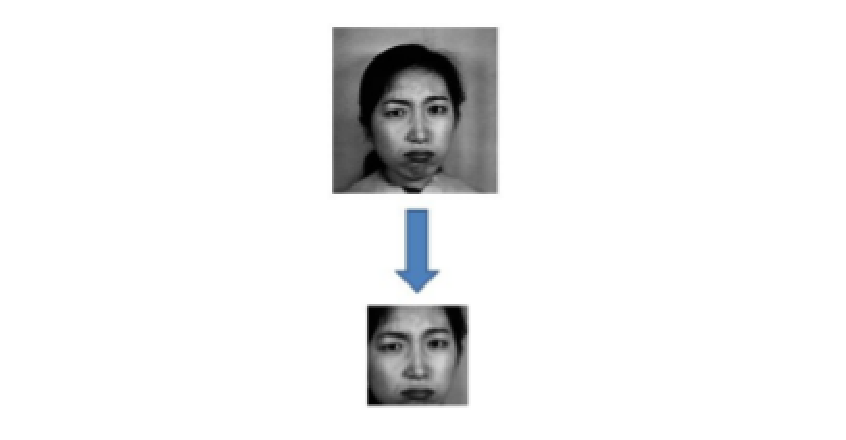
\includegraphics[scale=0.5]{graficos/rosto}
	\captionof{figure}{Detecção da face}
	\label{img:rosto}
	\cite{Elizabeth}
\end{center}
\item Extrair as principais características: Nesta etapa são extraídas as características que são relevantes à classificação da expressão. Normalmente é dada maior ênfase as sobrancelhas, nariz, olhos e boca. \ref{img:rosto_pontos}
A figura abaixo mostra a seleção de pontos mais relevantes para a classificação da expressão. 
\begin{center}
	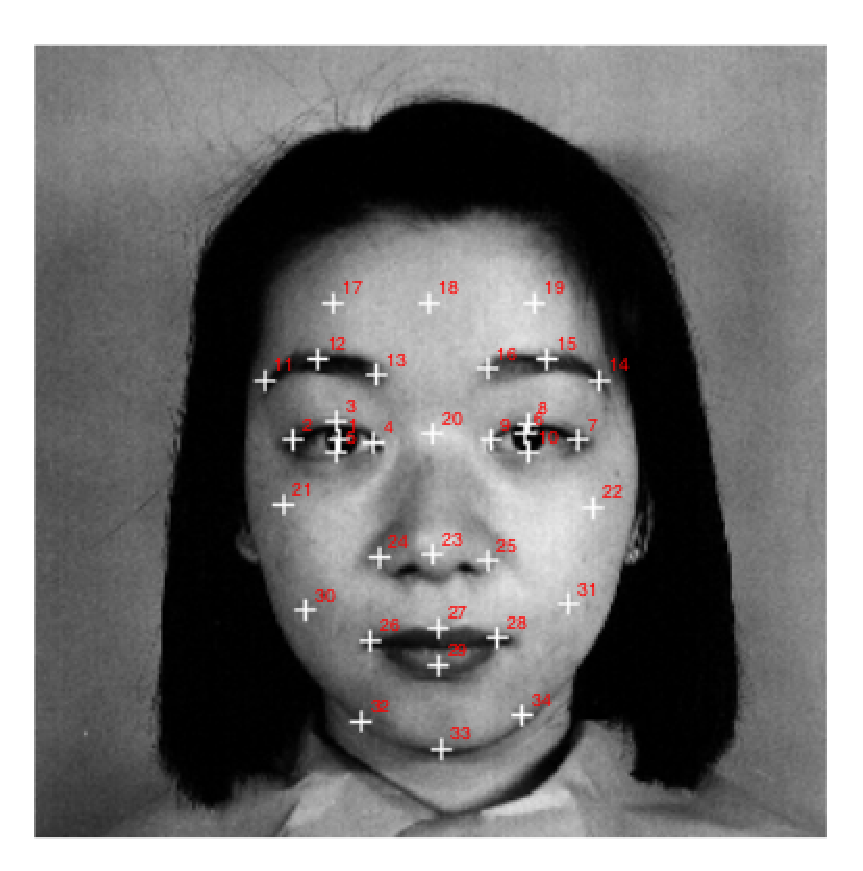
\includegraphics[scale=0.5]{graficos/rosto_pontos}
	\captionof{figure}{Pontos mais relevantes na face}
	\cite{Guo}
	\label{img:rosto_pontos}	
\end{center}
\item Classificar a imagem em uma detreminada expressão: Nesta etapa ocorre de fato a classificação da expressão. Para realizar esta classificação exitem diversos métodos, dos mais simples aos mais complexos. Alguns desse métodos serão apresentados na próxima seção.
\end{itemize} 

Na figura \ref{img:diagrama} está respresentado o processo de reconhecimento facial em suas três etapas básicas. No presente trabalho, a programação linear se aplica na etapa de classificação.
\begin{center}
	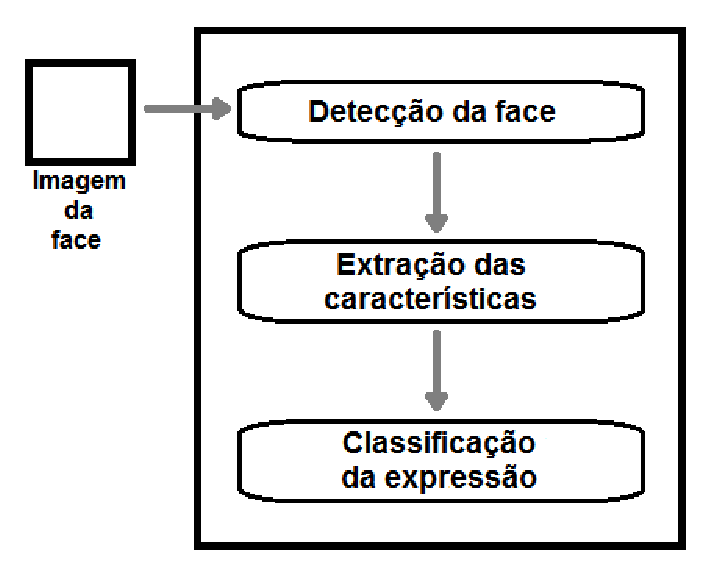
\includegraphics[scale=0.5]{graficos/diagrama}
	\captionof{figure}{Fases do processo de reconhecimento de expressão facial}
	\label{img:diagrama}	
\end{center}

\section{Métodos de Classificação}
Na últipa de etapa do processe de reconheicmento de expressões faciais, é realizada a classificação da expressão. Para a realização desta etapa existem diversos métodos. Alguns deles são apresentados nesta seção. Entre os métodos, existe aquele que utiliza a programação linear, principal fico deste trabalho, e que será apresentado na seção seguinte.

Em \cite{Hong} é descrito um método onde é utlizada uma base de dados com imagens de diferentes indivíduos relativas às expressões. A face a ser classificada é associada a face mais semelhante dentre as existentes na base dados, e após isso a expressão é classificada. Este método parte do princípio que pessoas com fisionomias semelhantes possuem uma maneira similar de apesentar a mesma expressão. Através de uma estrtura denominada General Face Knowledge são criados grafos sobre as imagens, através de pontos-chave da face. Quando o grafo do rosto, a ter sua expressão reconhecida, é criado, este é comparado aos grafos das imagens da base de dados, para que uma face semelhante seja encontrada. Na figura \ref{img:metodo1_classi} é ilustrado uma grfao sobre uma face. Esta abordagem obteve uma taxa de sucesso de cerca de 89\%.
\begin{center}
	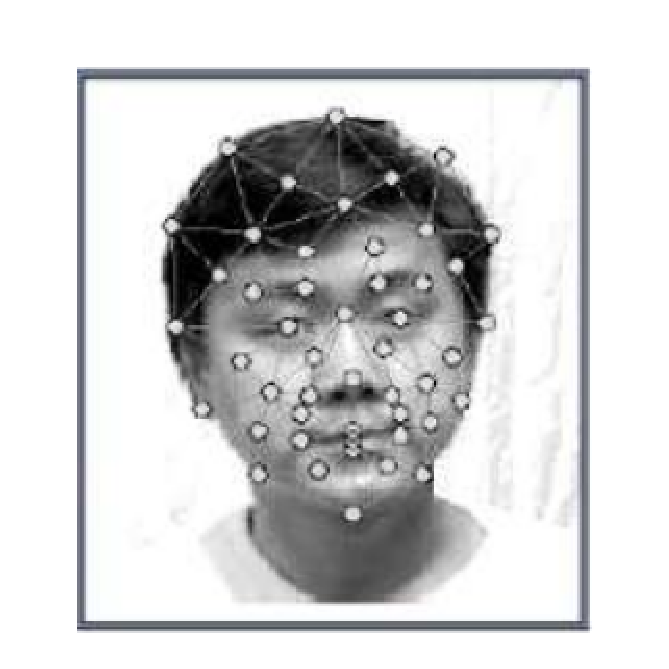
\includegraphics[scale=0.5]{graficos/metodo1_classi}
	\captionof{figure}{Exemplo de aplicação de General Face Knowledge ao rosto}
	\label{img:metodo1_classi}
\end{center}

\cite{Edwards} apresenta um outro método, em que é utilizado um framework denominado Active Appearance Models, nessa abordagem o objetivo é detectar a face idependente da luminosidade e posição. O  Active Appearance Models
possui um modelo estático que deve se ajustar a face que está sendo analisada através de alguns parâmetros e de forma iterativa. A figura \ref{img:metodo2_classi} ilustra o método.
\begin{center}
	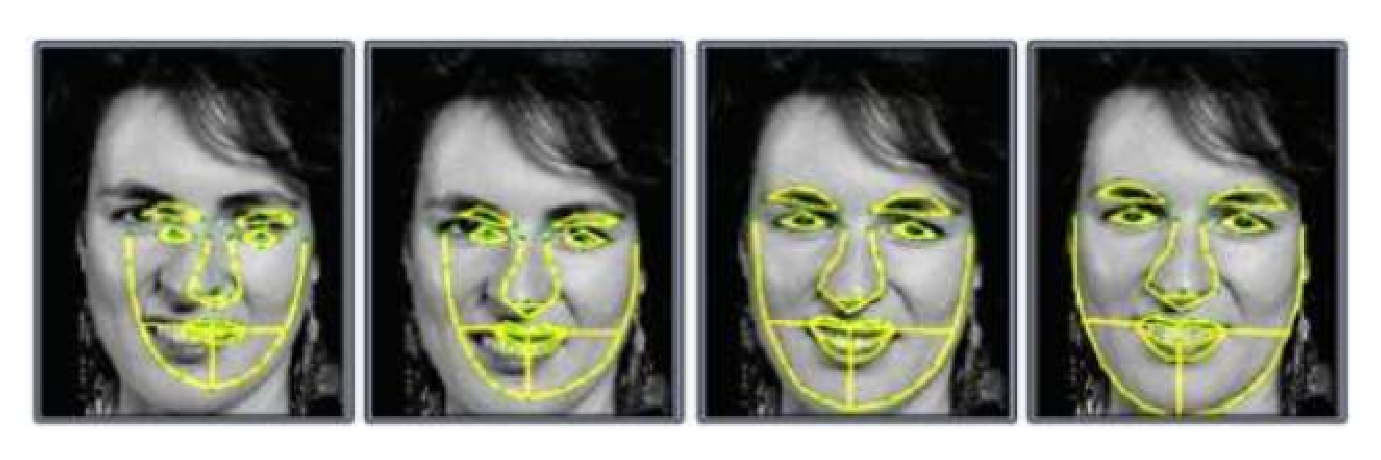
\includegraphics[scale=0.5]{graficos/metodo2_classi}
	\captionof{figure}{Ajuste do Active Appearence Models em três iterações a partir da posição inicial}
	\label{img:metodo2_classi}
\end{center}

Em um outro trabalho são definidas características-modelo, que são comparadas às características da face neutra, ou seja, sem expressar emoção, do indivíduo que está sendo analisao. Após essa etapa, é analisada a deformação, em relação ao modelo, quando o indivíduo expressa alguma emoção. A partir da deformação é realizada a classificação da expressão. A taxa de sucesso é de 92\% para a metade superior da face e de
86\% para a metade inferior. Na imagem \ref{img:metodo3_classi} é ilustrado o ajustamento das características modelo ao olho \cite{Pantic}.
\begin{center}
	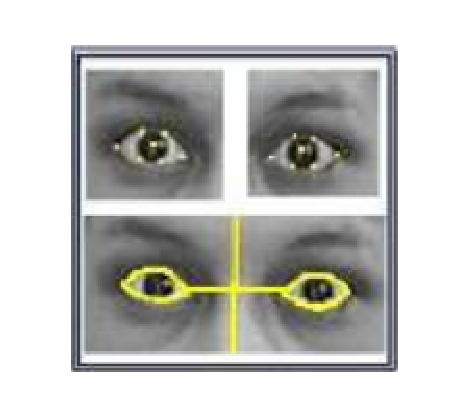
\includegraphics[scale=0.5]{graficos/metodo3_classi}
	\captionof{figure}{ Ajustamento ao olho: características-modelo}
	\label{img:metodo3_classi}
\end{center}

\section{O Reconhecimento de Expressões Faciais e a Programação Linear}

Em seus trabalhos, \citeonline{Feng} e \citeonline{Guo} apresentaram uma bordagem de reconhecimebto de expresssões faciais utilizando a progrmação linear. Em ambos a progrmação linear foi utilizada na fase de classificação da expressão. Em \citeonline{Guo} a programação lienar foi utlizada ainda na fase de extração de carcaterísticas, para determinar a quantidade de caracteríticas a serem selecionadas e os principais pontos da face. Enquanto no trabalho de \cite{Feng} é utilizado o filtro de Gabor na etapa de extração de carcaterísticas. O Filtro de Gabor tem a capacidade de realçar bordas e saliências na imagem. Após a aplicação do filtro na imagem, são realçadas as características salientes presentes no rosto (cantos dos olhos, cantos da boca, narinas, entre outros) \cite{Gabor}. Em ambos os trabalhos foram obtidos ótimos resultados e superiores a outros métodos com os quais foram comparados. 

A programação linear é utlizada na etapa após o tratamento da imagem. Primeiramente as expressões são combinadas em pares. No trabalho de \cite{Feng}, por exemplo, busca-se o reconhecimento de sete expressões: raiva, desgosto, medo, felicidade, tristeza, surpresa e neutro. Essas expressões são combinada em pares do tipo: raiva-desgosto, raiva-medo, etc. Formando um total de 21 pares. Após isso o modelo de programação linear, apresentado mais adiante, é utilizado para gerar os calssificares, o modelo deve ser rodado 21 vezes, uma para cada par de expressões. Essa etapa é também chamada de treinamento, pois a partir do classificadores gerados as expressões das imagens a serem analisadas serão determinadas. Essa abordagem também substitui a utilização de redes neurais para o treinamento, uma vantagem é que o modelo necessita ser rodado uma única vez para cada par, enquanto em uma abordagem utilizando redes neurais este processo se trona iterativo.

$Min\ \frac{e^{t}y}{m} + \frac{e^{t}z}{k}\\
\ subject\ to  \\
\              -A\omega + e\gamma + e <= y\\
\              B\omega - e\gamma + e <= z\\
\              y>= 0, z>= 0 $

Onde, 
\begin{itemize}
\item \textbf {$m$} representa a quantidade de imagens de rostos com a primeira expressão do par
\item \textbf {$k$} representa a quantidade de imagens de rostos com a segunda expressão do par
\item \textbf {$e$} é uma vetor de 1's
\item \textbf {$y$} e {$z$} são as varáveis do modelo
\item \textbf {$A$} é a matriz de pontos das imagens de rostos com a primeira expressão do par
\item \textbf {$B$} é a matriz de pontos das imagens de rostos com a segunda expressão do par
\end{itemize}

Na última etapa de determinação da exepressão é utilizda uma estrtura de árvore binária de torneio.

Através dessa arbordagem espera-se comprovar os ótimos resultados mostrados pelos trabalhos que utilizam a programação linear.

